%Packages
\documentclass{beamer}
\setbeamertemplate{footline}[frame number]
\usepackage{booktabs}
\usepackage{xcolor}
\usepackage{graphicx}
\usepackage{subcaption} % Ensure this is compatible with Beamer
\usepackage{multirow}
\setlength{\tabcolsep}{4pt} % Adjust the column padding
\usepackage{makecell}
\usetheme{Boadilla} % Feel free to change the theme to suit your style
\usepackage{verbatim}
\usepackage{natbib}


% Title, authors, and institutions
\title[Work in Progress]{Higher Education Access Disparities in Portugal}
\author[M. Sousa Duarte, V. Conde Mendes] % Shortened author names for the footer
{
  Miguel Sousa Duarte\inst{1} and Vicente Conde Mendes\inst{2}
}
\institute[]{
  \inst{1} Copenhagen Business School \\
  \inst{2} École Polytechnique Fédérale de Lausanne
}
\date{WIP Seminar \textendash\ \today }


%Begin document
\begin{document}
\begin{frame}
  \titlepage
\end{frame}
\begin{frame}{Table of Contents}
  \tableofcontents
\end{frame}


\section{Motivation}

\begin{frame}{Motivation: Private Schools Grade Inflation}
\begin{itemize}
    \item 25\% of high school (HS) students attend private institutions.
    \item Private HS students achieve higher grades both on school-internal grading and on National Exams (NE)
    \item The ten 10 HS with the greater difference between internal grading and NE grade are private \citep{sapo2024}.
\end{itemize}
\begin{figure}
    \centering
    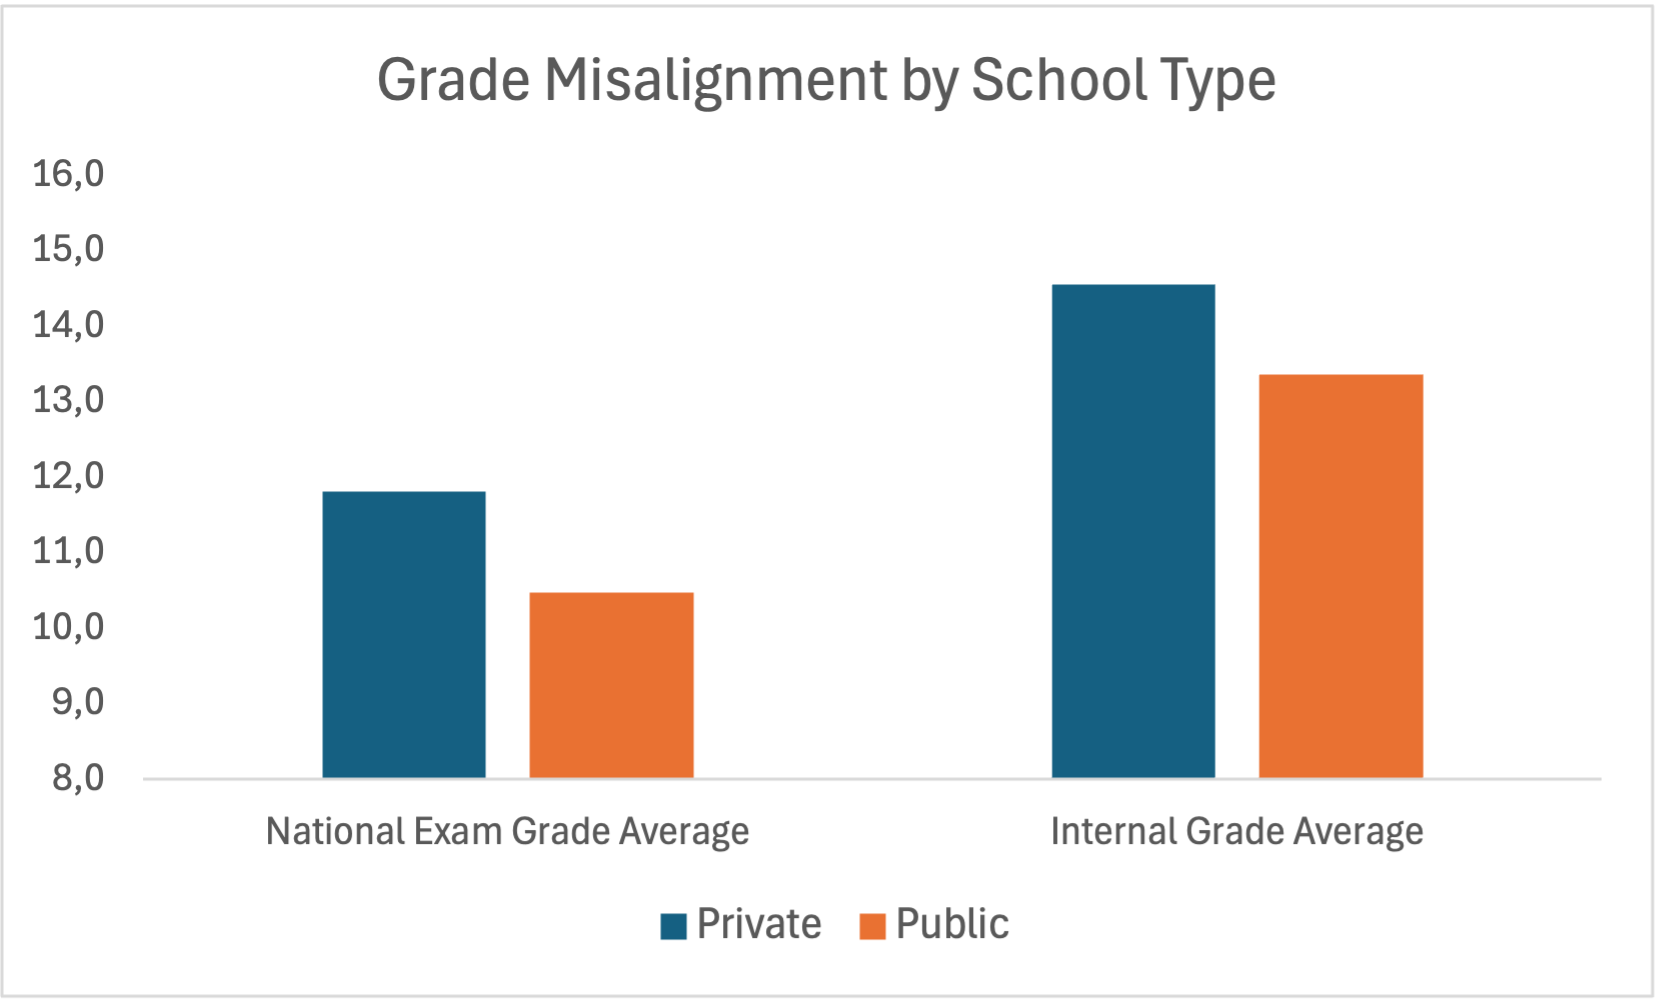
\includegraphics[width=0.5\linewidth]{Figures/InflationBySchoolTypeOurs.png}
    \caption{Inflation by school type}
    \label{fig:InflationBySchoolTypeOurs}
\end{figure}
\end{frame} 


\begin{frame}{Persistence over the Years}

\begin{table}[ht]
\centering
\caption{Spearman Rank Correlation of School Grade Inflation by Year}
\label{tab:spearman_corr}
\begin{tabular}{l *{8}c}
\toprule
 & \multicolumn{1}{c}{2014} & \multicolumn{1}{c}{2015} & \multicolumn{1}{c}{2016} & \multicolumn{1}{c}{2017} & \multicolumn{1}{c}{2018} & \multicolumn{1}{c}{2019} & \multicolumn{1}{c}{2022} & \multicolumn{1}{c}{2023} \\
\midrule
2014 & 1.000  &         &         &         &         &         &         &         \\
2015 & 0.733\textsuperscript{*} & 1.000  &         &         &         &         &         &         \\
2016 & 0.576\textsuperscript{*} & 0.640\textsuperscript{*} & 1.000  &         &         &         &         &         \\
2017 & 0.681\textsuperscript{*} & 0.769\textsuperscript{*} & 0.641\textsuperscript{*} & 1.000  &         &         &         &         \\
2018 & 0.609\textsuperscript{*} & 0.707\textsuperscript{*} & 0.612\textsuperscript{*} & 0.793\textsuperscript{*} & 1.000  &         &         &         \\
2019 & 0.608\textsuperscript{*} & 0.723\textsuperscript{*} & 0.592\textsuperscript{*} & 0.747\textsuperscript{*} & 0.819\textsuperscript{*} & 1.000  &         &         \\
2022 & 0.450\textsuperscript{*} & 0.534\textsuperscript{*} & 0.484\textsuperscript{*} & 0.601\textsuperscript{*} & 0.696\textsuperscript{*} & 0.757\textsuperscript{*} & 1.000  &         \\
2023 & 0.422\textsuperscript{*} & 0.456\textsuperscript{*} & 0.404\textsuperscript{*} & 0.498\textsuperscript{*} & 0.556\textsuperscript{*} & 0.612\textsuperscript{*} & 0.726\textsuperscript{*} & 1.000  \\
\bottomrule
\end{tabular}

\vspace{0.5em}
\raggedright
\textsuperscript{*}\,Significant at the 1\% level.
\end{table}
\end{frame} 

\begin{frame}{Three types of schools}
  \begin{figure}[ht]
  \centering
  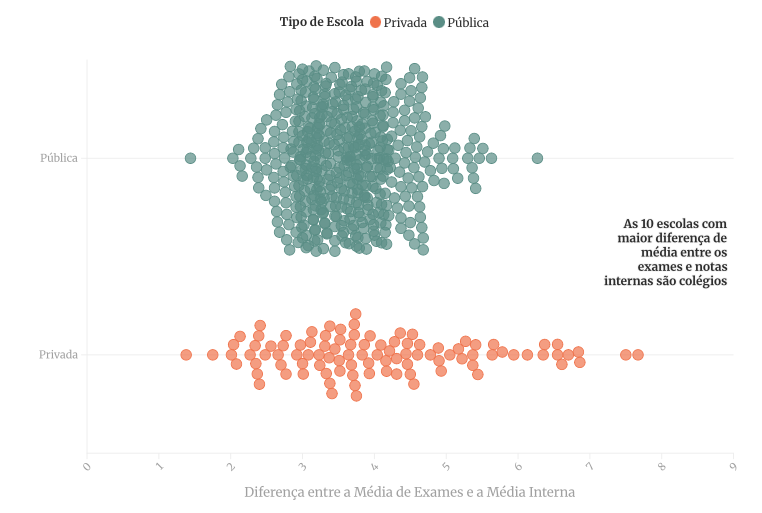
\includegraphics[height=5cm, keepaspectratio]{Figures/InflationBySchoolNEW.png}
  \caption{Inflation by Individual School}
  \label{fig: InflationBySchoolNEW}
\end{figure}
\end{frame} 


\section{Public University Application Process}

\begin{frame}{Public University Application Process: Rules}
    Application grade is often composed by 50\% of school-given internal grade and 50\% of national exams relevant for the BSc programme.
    \begin{itemize}
        \item National exams are provided and corrected by the central government.
        \item The exact proportion and which national exams are relevant is defined by the university.
    \end{itemize}

    Note that final internal grade is also dependent on national exams. By government rule, for each subject, the internal grade is 70\% teacher's grade and 30\% national exam grade.
     \begin{itemize}
        \item \textbf{Key: Schools' internal grading play a relevant role in university application GPA, in a system in which this is the only qualifying mechanism.}
        \item Students rank their 6 programmes of choice when applying to university.
    \end{itemize}
    
\end{frame}

\begin{frame}{Public University Application Process: Example}
\begin{tabular}{|lcccccc|}
\hline
 & \makecell{Internal \\ Grade} & BSc & \makecell{Biology \\NE} & \makecell{Physics \\NE} & \makecell{Maths \\NE} & \makecell{Application \\ Grade} \\
\hline
\multirow{3}{*}{Emma} & 15 & Medicine & 13 & 20 & 11 & 14.8 \\
 & 15 & Economics & - & - & 11 & \textbf{13} \\
 & 15 & Psychology & 13 & - & 11 & 13.5 \\
\hline
\multirow{3}{*}{Ricky} & 14 & Medicine & 19 & 20 & 11 &\textbf{15.3} \\
 & 14 & Economics & - & - & 11 & 12.5 \\
 & 14 & Psychology & 19 & - & 11 & \textbf{14.5} \\
\hline
\end{tabular}
\begin{itemize}
    \item Emma and Ricky are considering the same 3 bachelor programmes.
    \item The two classmates have different internal final grade and Biology National exam grade
    \item Emma would get in front of Ricky into the Economics program but behind him in Medicine and Psychology.
\end{itemize}
\end{frame}


\section{Methodology}

\begin{frame}{Methodology}
  \begin{itemize}
    \item For each subject that is subject to a national exam:
    \begin{itemize}
        \item Find the average grade inflation per school.
    \end{itemize}
  \end{itemize}
  \begin{figure}[ht]
  \centering
  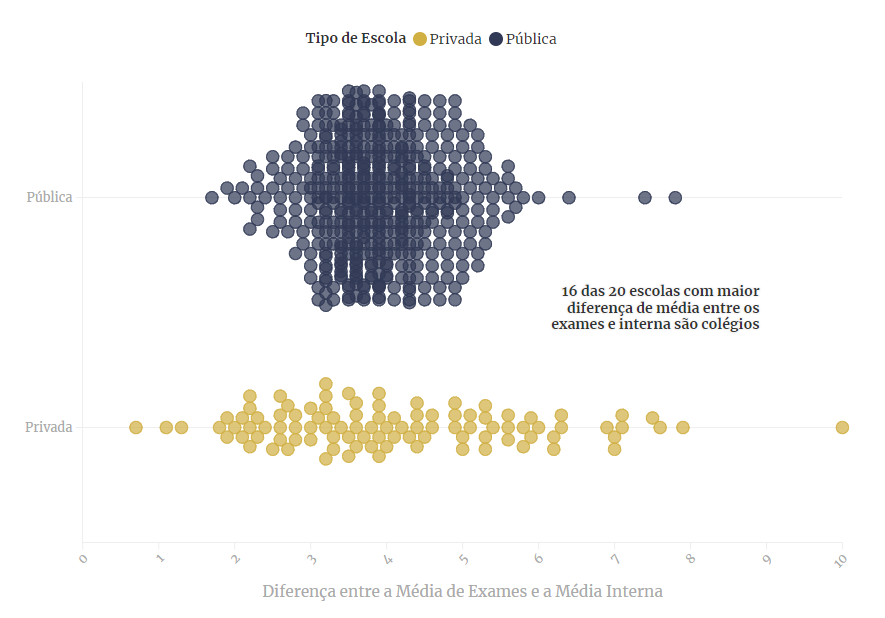
\includegraphics[height=5cm, keepaspectratio]{Figures/InflationBySchool.png}
  \caption{Inflation by Individual School}
  \label{fig: InflationBySchool}
\end{figure}
\end{frame}

\begin{frame}{Methodology}
    \begin{itemize}
    \item For each subject that is subject to a national exam find the average grade inflation per school.
    \item With individual-level data, re-compute the final grade with which the student applies to university with.
\end{itemize}


  \begin{block}{Adjusted Subject Internal Grade}
  \begin{align}
\text{Adj.Grade} = \text{Internal Grade} -\text{Subject School-Specific Grade Inflation}
  \end{align}
  \end{block}
  
% \begin{block}{Adjusted Grade}
%  \begin{align}
%    \text{Ajd.Grade} = \text{Final Grade} -\text{School-Specific Grade Inflation}
%  \end{align}
% \end{block}

\begin{itemize}
    \item The Adjusted Final Internal Grade then is computed by using the Adjusted Grades from the subjects in which the student was subject to exam, together with the original internal ones for subjects the student did not sit in for in a national exam.
\end{itemize}

\end{frame}

\begin{frame}{Grade Adjustment: Example}
    Let us consider Emma and her Biology subject.
    
\begin{table}[h!]
\centering
\begin{tabular}{|l|c|}
\hline
Country Misperformance & 2.91 \\ \hline
School Misperformance  & 3.47 \\ \hline
Internal Grade         & 17 \\ \hline
Exam Grade             & 12.9 \\ \hline
Final Official Grade   & 15.77 \\ \hline
\end{tabular}
\caption{Grades and Misperformance Data}
\end{table}

Emma's teacher graded her with a 17. Emma scored a 12.9 in the national exam. Her final grade was  $70\% \cdot 17+30\% \cdot 12.9=15.77$ 

Her internal grade is then adjusted to account for school-specific Biology grade inflation: 
\[\text{Adj.Grade}=70\% \cdot [17-(3.47-2.91)]+30\% \cdot 12.9 = 15.38\]



% In the overall country, students sitting in for the Biology exam, scored 2.91 points below their internal grade. In Emma's school, this figure was 3.47. Emmma's teacher gave her an 17 for her in-class performance. Emma scored a 12.9 in the national exam. Her final grade in Biology then was $70\%*17+30\%*12.9=15.77$

\end{frame}

\begin{frame}{Methodology}
    \begin{itemize}
    \item Find the average grade inflation per school.
    \item With individual-level data, re-compute the grade with which the student applies to university with.
    \item Re-assess the admissions of students into study programmes in a simulated setting where grades are inflation-adjusted.
    %Having data on the 6 preferences the student enumerates when applying to public university, re-assess the distribution of students in a simulated setting where grades are inflation-adjusted?
    \begin{itemize}
        \item \textbf{Does the proportion of public high school students in high grade requirement courses  increase upon this adjustment?}
    \end{itemize} 
\end{itemize}

\end{frame}



\section{Discussion of Method and Handicaps}
\begin{frame}{Method: Grade Adjustment}
    \begin{itemize}
        \item If Emma scores higher in the National Exam than in the internal grade, does it make sense to adjust her grade downwards due to school inflation?   
    \end{itemize}
    
\end{frame}

\begin{frame}{Extensions}
    \begin{itemize}
        \item Some subjects, like Physical Education and senior year electives, are not subject to exam yet count for the internal grade. What's more, the data shows that private schools award higher grades on these subjects. How to \textit{adjust} for this?
        \begin{itemize}
            \item Physical Education only recently became part of the internal grade, so one can study the impact of its introduction.
        \end{itemize}
        \item Covid period:
        \begin{itemize}
            \item Exams were easier: Graded out of 20 but with 20+ possible points.
            \item Fewer exams: Only sitting in if needed for university application.
            \begin{itemize}
                \item Greater relevance of internal grades!
            \end{itemize} 
        \end{itemize}
       
    \end{itemize}
    
\end{frame}

\begin{frame}{Method: Grade Adjustment Alternative}
   
\begin{itemize}
    \item Revisiting Emma and her Biology subject:
\end{itemize}
    
\begin{table}[h!]
\centering
\begin{tabular}{|l|c|}
\hline
Country Misperformance & 2.91 \\ \hline
School Misperformance  & 3.47 \\ \hline
Internal Grade         & 17 \\ \hline
Exam Grade             & 12.9 \\ \hline
Final Official Grade   & 15.77 \\ \hline
\end{tabular}
%\caption{Grades and Misperformance Data}
\end{table} 

Could one say that since $\text{Exam}-\text{Internal}>\text{School Misperformance}$, the grade should in fact be adjusted to:
\[70\% \cdot [17-(17-12.9-2.91)]+30\% \cdot 12.9 = 14.94 \]

However, this completely foregoes the school-type perspective.
    
\end{frame}

\begin{frame}{Handicaps}

\textbf{Data Availability:} The data is from an Education Directorate. As such, it is unlikely that there will be extensive data on the individual. Harder to control for income, for example. Best alternative: Proxy by wealth in the municipality of the school.     
\end{frame}


\begin{frame}{Top-up: Labour Market Outcomes}

\begin{itemize}
    \item Make a collection of all pairs of students with:
    \begin{itemize}
        \item Same national exam scores
        \item Same preferences for university
        \item Different schools
        \item Different outcomes from university application due to internal grading
    \end{itemize}
    \item Evaluate the discrepancy in the labour market outcome of the students.    
\end{itemize}

\textbf{Concern:} Up until now, all information could be sourced from the  Directorate-General for Statistics of Education and Science (DGEEC). Labour market outcomes most certainly requires a different source of information (DST/INE or social security), thereby requiring asking the institutions to merge their datasets and then make them available to us with anonymity.
   
\end{frame}

\begin{frame}{Bibliography}
\bibliographystyle{apalike}
\bibliography{references}    
\end{frame}



\begin{comment}
\begin{frame}{Inflation analysis}
    \begin{itemize}
    \item Average inflation per type of school, with distribution (how wide, for each type of school?).
    \item inflation per subject
    \item inflation per region of the country
    \item evolution of measures of inflation over the years
    \end{itemize}
\end{frame}
\end{comment}

\end{document}